\documentclass [notitlepage, 12pt, a4paper]{article}
\usepackage[a4paper, portrait, margin=1in]{geometry}
\usepackage[articletitle=false,etalmode=firstonly,maxauthors=3]{achemso}
\usepackage{csquotes}
\usepackage{amsmath}
\usepackage{mathptmx}% http://ctan.org/pkg/mathptmx
\usepackage{enumitem}
\usepackage{hyperref}
\usepackage{graphicx}
\usepackage[parfill]{parskip}

% Default fixed font does not support bold face
\DeclareFixedFont{\ttb}{T1}{txtt}{bx}{n}{12} % for bold
\DeclareFixedFont{\ttm}{T1}{txtt}{m}{n}{12}  % for normal

% Custom colors
\usepackage{color}
\definecolor{deepblue}{rgb}{0,0,0.5}
\definecolor{deepred}{rgb}{0.6,0,0}
\definecolor{deepgreen}{rgb}{0,0.5,0}
\definecolor{mygray}{rgb}{0.4,0.4,0.4}

\usepackage{listings}

% Python style for highlighting
\newcommand\pythonstyle{\lstset{
language=Python,
basicstyle=\ttm,
keywords={self, def, while, return, if, else, from, import, raise},             % Add keywords here
keywordstyle=\ttb\color{deepblue},
emph={MyClass,__init__, ValueError},          % Custom highlighting
emphstyle=\ttb\color{deepred},    % Custom highlighting style
stringstyle=\color{deepgreen},
frame=tb,                         % Any extra options here
showstringspaces=false,            %
commentstyle=\color{mygray}
}}

% Python environment
\lstnewenvironment{python}[1][]
{
\pythonstyle
\lstset{#1}
}
{}
\newcommand\pythoninline[1]{{\pythonstyle\lstinline!#1!}}

\begin{document}

\title{ASE Task and Workflow Description}

\section{Class Structure}

\subsection{Task}
A task is an object that can take in a set of generalized inputs, and use a given evaluator function to calculate a set of desired outputs.
This should represent a single DFT or similar calculation.

\subsubsection{Members}
input structure: A structure that stores the input variables for the evaluator

evaluator function: A function object that sets up, runs, and post processes the calculations to get a desired output

results: A data structure that stores the desired outputs (probably a dictionary will be easiest)

logfile: an optional log file path (storage for things like output files from DFT or evaluation data if the user wants it). The evaluator should control any potential logging

\subsubsection{Functions}
\begin{python}
def __init__(self, inputs, evaluator, logfile=''):
    self.inputs = inputs
    self.evaluator = evaluator
    self.logfile = logfile
    self.results = {}
\end{python}
This function initializes the data structures and the evaluator function.

\begin{python}
def get_result(self, key=''):
    if(key == ''):
        return the full dictionary
    else:
        return results[key]
\end{python}
The actual code can change to match the results data structure.

\begin{python}
def run():
    use inputs to prepare the desired (list of)
    calculation(s) as a list of tasks
    (len(task) == 1 is possible)
    evaluator(tasks)
\end{python}
Not strictly needed as evaluator(inputs) would also work just as well inside a main python function

\subsection{Workflow}
A workflow is a class (potentially a superclass where more specialized workflows can be later derived from) that can generate and manage a set of tasks to reach a user defined final state or get a defined output value.
The workflow should take in (if we use a superclass define virtual functions for) the initial task inputs/evaluator functions as well as methods to mutate the inputs to get to the final results and define the convergence criteria.
The user will have to also input a representation of the dependency graph so the work flow can map out/visualize what it is doing.
The final result as well as all the individual task results should be accessible to the user in a standardized format.
If the individual task results are not needed a flag can be used to discard them.
\subsubsection{Members}
    graph: A standardized description of the workflow that can be used to generate a dependency graph for the individual tasks. The actual structure of this should be standardized and easy for a user to create either by a utility function or by hand

    taskStorage: A data structure that stores the tasks that have been created by the work flow. This structure should be flexible enough to add a series of them while running if only a convergence criteria is known and not the total number of calculations. It can also be used as a proto super trajectory class.

    results: The final result of the work flow. It should use the results from the individual tasks to calculate a final outputs

    lossFxn: While running the code this function tells the workflow when a series of tasks is completed. This could be a list if there are multiple steps.

    baseEvaluator: The evaluator functions for the tasks. This could be a list if there are multiple steps

    initialInputs: Description of the initial inputs that will be modified by a function to generate each task in the work flow. This could be a list if there are multiple steps

    changeInputsFunction: A function that updates initialInputs as the results converge. (This may just have to be hard coded into the workflow functions)

    logfile: Optional file that gives a more detailed description of what the workflow is doing
\subsubsection{Functions}
\begin{python}
def __init__(self, graph, lossFxn, baseEvaluator, initialInputs,
             changeInputsFunction, logfile=''):
    self.graph = graph
    self.lossFxn = lossFxn
    self.baseEvaluator = baseEvaluator
    self.initialInputs = initialInputs
    self.changeInputsFunction = changesInputsFunction
    taskStorage = []
    results = {}

\end{python}
Initializes all members and evalutor functions

\begin{python}
def setup(self):
    - Read Graph
    - Setup taskStorage using correct functions
\end{python}
Read in the graph describing the work flow and initialize the task generation and storage.

\begin{python}
def run(self)
    while(lossFxn returns false):
        - Modify inputs using changeInputsFunction
        - Create tasks and store them in taskStorage
        - Determine how to run/monitor the tasks/individual
          calculations
\end{python}
The checking the individual calculations will be a challenge and where FireWorks maybe incorporated.
Controls between steps will also be necessary

\begin{python}
def getResults(self, flag deciding whether to use task/workflow
               results ):
    Return the final results or the individual task results
    depending on what how the final results are stored
\end{python}
Largely based on how we store the results.

\begin{python}
def show_graph(self):
    somehow reflect the internal dependency structure
\end{python}
We should see if there are math libraries that can do this for us.

\subsection{Difference Between Task and Workflow}
\begin{itemize}
\item Task has no internal dependencies, only depends on generalized input and a single function call (sth. a user would submit to the queue as a job or a single DFT calculation)
\item Workflows can have a nested dependency structure with serial and parallel dependencies:
\item Example: Geometry relaxation\\
In each step, a task ‘get\_forces’ needs to performed to allow the optimizer to predict a new geometry
\item \textcolor{deepred}{REM: Maybe a unified Task/Workflow class is sufficient to achieve this?}
\end{itemize}

\subsection{List of potential tasks and workflows with pseudo input}

\begin{python}
# return: atoms object with results
def SinglePointCalculation( input_atoms, input_calc, evaluate):
    return atoms_claculated
\end{python}

\begin{python}
# aglorithm: Some general iterator that yields new atoms until
# convergence
# return: atoms and calculator with optimized values
def Optimizer(input_atoms, input_calc,
              algorithm(loss_fct<1e-3), evaluate):
    return optimized_atoms, optimized_calc
\end{python}

\begin{python}
# return: PhonopyObject with forces calculated
def Phonopy(input_atoms, input_calc, {disp=0.01,
            supercell=[-2, 2, 2, 2, -2, 2, 2, 2, -2], **kwargs},
            evaluate)
    return PhonopyObject
\end{python}

\begin{python}
# A function that will be generalized to several different tasks
# like BandStructure, DOS, ThermalProperties, ...
# return: desired phonon property
def PhonopyPostprocess(PhonopyObject, {q_mesh=[15, 15, 15],
                       q_points='default', **kwargs}, evaluate)
    return  phononProp
\end{python}

\begin{python}
# return: Phono3pyObject with forces calculated
def Phono3py(input_atoms, input_calc, {fc2_disp=0.01,
             fc3_disp=0.03, cutoff=2.0,
             fc2_supercell=[-2, 2, 2, 2, -2, 2, 2, 2, -2],
             fc3_supercell=[-1, 1, 1, 1, -1, 1, 1, 1, -1],
             **kwargs}, evaluate)
    return  Phono3pyObject
\end{python}

\begin{python}
# return: desired property, e.g. thermal conductivity
def Phono3pyPostprocess(Phono3pyObject, {q_mesh=[15, 15, 15],
                        q_points='default', **kwargs})
    return prop
\end{python}

\begin{python}
# return: A list of atoms with some extras
def StatisticalSampling(inital_atoms, initial_calc,
        force_constants, SamplignDriver (creates configurations),
        RandomNumberGenerator, NSamples='default')
    return Trajectory
\end{python}

\begin{python}
# return: A list of atoms with some extras
def MD(input_atoms, input_calc, MD_driver,
        timestep='default', runtime='default', evaluate)
    return Trajectory
\end{python}
\newpage
\begin{python}
# return: A list of atoms containing the subset of atoms that
# have the stresses computed
def StressMD(input_atoms, input_calc, MD_driver,
        timestep='default', runtime='default', evaluate)
    return Trajectory
\end{python}

\begin{python}
# return: Thermal conductivity + X
def GreenKubo(MDTrajectory with computed stresses, {**kwargs})
    return Thermal conductivity + X
\end{python}

\section{Pseudo Code of Phononpy Calculation with Postprocessing Tasks}
\begin{figure}
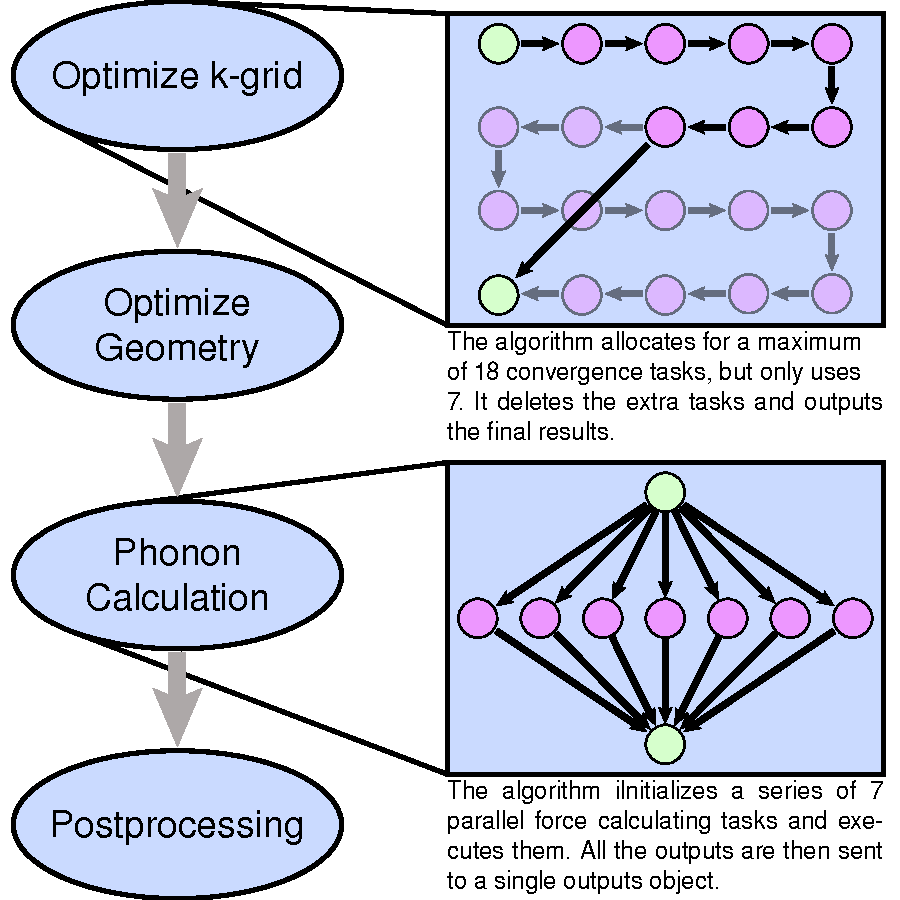
\includegraphics{PhonnWorkflowDiagram.pdf}
\caption{Schematic of the dependency graph calculated or given to the system.}
\label{fig:depGraph}
\end{figure}
\subsection{Workflow.py}
\begin{python}
import * from HiLDeWorkflowLib
import numpy as np
from ase import atoms, .....
import evaluate from HiLDeEvaluationFunctionLib
input_atoms = ase.atoms()
input_calc  = ase.calculator()

# You'd input the graph so the code would be able to generate this
# process as a task structure. Each one of the function calls
# would be defined as a separate task described in the
# taskStructure. I have them listed as a python script here for ease
# of interpretation

# The workflow will have to change slightly since the functions
# objects listed there are stored within the task's functions
# themselves

optKGridAtoms, optKGridCalc = Optimizer(input_atoms, input_calc,
                              kGridOpt(loss_fct<1e-3), evaluate)
relaxedGeoCalc = optKGridCalc.make_geometry_relaxation()
relaxedAtoms = SinglePointCalculation(optKGridAtoms, relaxGeoCalc,
               evaluate)
phonoCalc = relaxGeoCalc.make_phonon_calc()
phonopyObject = Phonopy(relaxedAtoms, phonoCalc, {disp=0.01,
                supercell=[-2, 2, 2, 2, -2, 2, 2, 2, -2], **kwargs},
                evaluate)
results['property'] = PhonopyPostprocess(phonopyObject,
                      {q_mesh=[15, 15, 15], q_points='default',
                      **kwargs}, evaluate)
\end{python}
\newpage
\subsection{Optimizer Layout}
\begin{python}
def atomsGenerator(atoms, calc):
    if(convergence criteria is met):
        yield None
    else:
        yield newAtoms, newCalc
def Optimize(atoms, calc, nMax, atomsGenerator):
    for nn in range(nMax):
        Make task to do single point calculation on atoms/calc
        new_atoms, new_calc = atomsGenerator.send(atoms, calc)
        if(new_atoms is not None):
            atoms, calc = new_atoms, new_calc
        else
            return atoms, calc
    raise ValueError("exceeded maximum number of steps")
\end{python}

\subsection{Optimize Geometry}
This can be taken from HighAims task library (all single point calculations will be similar)

\subsection{Phonopy Object}
\begin{python}
def Phonopy(atoms, calc, {disp=0.01,
            supercell=[-2, 2, 2, 2, -2, 2, 2, 2, -2], **kwargs},
            evaluate):
    # Set up the phonopy object and displacements as normal
    for disp in dispList:
        setup/make task for each disp, and execute the task
    Wait until all tasks are finished and incorporate them into the
    phonopyObject
\end{python}

\subsection{Postprocessing}
This will be a collection of tasks to get the final results you want from the workflow.
Most of these can be pulled from previously written postprocessing steps.

\section{Database Structure}
Tasks and Workflows (generalized tasks) should be able to hash itself as hashes of the inputs

\section{Initial Example to be Completed}
Example application: Optimize geometry and perform phonon calculation
- Ask

\section{Loose List of Ideas}
\begin{itemize}
    \item \emph{hash.ini} file stores the keys are (not) to be hashed
\end{itemize}

\end{document}